\documentclass[10pt]{beamer}

\usepackage{appendixnumberbeamer}

\usepackage{booktabs}
\usepackage[scale=2]{ccicons}

\usepackage{pgfplots}
\usepgfplotslibrary{dateplot}

\usepackage{xspace}
\usepackage{../theme_style}
\setbeameroption{show notes}

\title[Leader Election and Consistency]{Exam question two - Leader Election and Consistency}
\subtitle{Distributed and Pervasive Systems}
\date{June 03, 2022}
\author[M.H. Kristensen]{Morten Haahr Kristensen}
\def\studentid{201807664}
\institute{Department of Electrical and Computer Engineering - Aarhus University}
% Logo only on title page
\titlegraphic{
    
\includegraphics[width=12cm]{figs/aulogo_big.png}
}
\begin{document}

\maketitle

\begin{frame}{Outline}
  \setbeamertemplate{section in toc}[sections numbered]
  \tableofcontents[hideallsubsections]
\end{frame}


\section{Motivation}

\begin{frame}{Motivation}
  \begin{alertblock}{Distributed System definition \cite{vansteenDistributedSystems2018}}
    A distributed system is a collection of autonomous computing elements that \textbf{appears} to its users as \textbf{a single coherent system}.
  \end{alertblock}
  \begin{itemize}
    \item In order for systems to appear as a single coherent system the different processes in the system must agree on the state.
    \note[item]{
      This leads us to the topic of consistency. The state must be consistent across nodes.
    }
    \item Distributed systems allow for horizontal scaling. However, we may need a coordinator for the nodes to cooperate properly.
    \note[item]{
      A leader's role often includes being the organizer of a system.\\
      This could be in regards to fault tolerance. E.g. the first phase of RAFT is to select a leader.
    }
  \end{itemize}
\end{frame}

\section{Consistency}
\begin{frame}
  \frametitle{Replication}
  Replicate data among nodes to ensure:
  \begin{itemize}
    \item Reliability
    \item Load balancing
    \item Geo scaling
  \end{itemize}
  The tradeoff is that we introduce consistency problems.
  \note{
    When talking about these things compare them to a centralized system.
  }
\end{frame}

\begin{frame}
  \frametitle{Definitions}
  \begin{alertblock}{Consistency \cite{pedersenConsistencyDistributedPervasive2022}}
    All nodes in the system agree on the current state.\note[item]{
      We will elaborate further on the consistency definition later, as it turns out that there are different levels of consistency guarantees.
    }
  \end{alertblock}
  \begin{alertblock}{Availability \cite{pedersenConsistencyDistributedPervasive2022}}
    The system is operational and instantly processing incoming requests.\note[item]{
      I have also seen it defined as every request receives a (non-error) response. I like that better because it avoids ''instantly''.
    }
  \end{alertblock}
  \begin{alertblock}{Partition tolerance \cite{pedersenConsistencyDistributedPervasive2022}}
    Partition tolerance is the ability of a distributed system to continue operating correctly event in the presence of a network partition.
  \end{alertblock}
  \note[item]{A network partition is a failure where a network splits into at least two parts that cannot communicate with each other.}
\end{frame}

\begin{frame}
  \frametitle{CAP}
  \metroset{block=fill}
  \begin{alertblock}{CAP \cite{pedersenConsistencyDistributedPervasive2022}}
    If there is a network \textbf{P}artition, the system must choose between \textbf{A}vailability and \textbf{C}onsistency.
  \end{alertblock}
  \note[item]{
    Give the example with CAP:\\
    Two nodes sharing some state. A network partition happens so they can't communicate. Something triggers one of the nodes to change their common state. It can either:
    \begin{enumerate}
      \item Update its local state and make them inconsistent
      \item Not update its state and make the system unavailable for updates.
    \end{enumerate}
  }
  \begin{figure}
    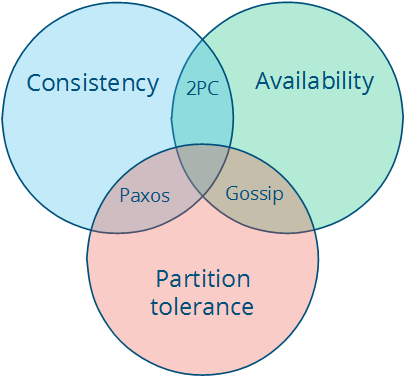
\includegraphics[width=0.45\textwidth]{figs/cap_overview.png}
    \caption{Overview of CAP. Center is not achievable. \cite{takadaDistributedSystemsFun2013}}
  \end{figure}
  \note[item]{So we can either have a CA system, a CP system or an AP system.}
  \note[item]{Examples of CA systems: Traditional relational databases like MySQL, Postgres etc. Here we cannot tolerate network partitions and must stop accepting writes in case a node fails.}
  \note[item]{Examples of AP systems: Apache Cassandra. We don't guarantee consistency among our network partitions.}
  \note[item]{Examples of CP systems: MongoDB. Here we only allow one of our partitions to be written to. This gives us a certain degree of availability and provides full consistency.}  
\end{frame}
\note{It should be clear now that is very application specific which type of system to implement. Example:
\begin{itemize}
  \item Facebook likes on a post. It might not be that important whether the user sees 350 or 351 likes on a post. AP is probably fine.
  \item Banking systems. A user's bank account must be consistent among the servers. This can either be a CA or CP system. Probably CP since otherwise, their entire "Netbank" will be down for writes in case of a network partition. Then it is better to provide some degree of service (while it may be slower) over no service.
\end{itemize}}

\begin{frame}
  \frametitle{Strong consistency model}
  \begin{alertblock}{Strong consistency\footnote{The definition is paraphrased from: \cite{pedersenConsistencyDistributedPervasive2022}}}
  An update is \textbf{immediately} propagated to all other nodes. If two updates happen concurrently, the updates must be processed in the \textbf{same order} at all nodes.\\
  Strong consistency guarantees that the system is in a \textbf{consistent state} when a transaction has finished and before the next transaction can be handled.
  \end{alertblock}
  \note[item]{So with strong consistency we have this strong guarantee that our data is consistent among the different nodes at any given time. An update is not committed fully until it has been propagated to all nodes. This also provides a reading guarantee that no matter which node we read from it will be in a consistent state.}
  \note[item]{The downside is obviously latency. If we need to send messages to each node whenever we make a change, the system becomes more unresponsive to the user. We talk more about this later.}
\end{frame}

\begin{frame}
  \frametitle{Weak consistency model}
  \begin{alertblock}{Eventual consistency \cite{pedersenConsistencyDistributedPervasive2022}}
    Eventual consistency guarantees that the state is eventually agreed upon but the nodes may temporarily disagree.
  \end{alertblock}
  \note[item]{DNS servers are probably the most known example of an eventually consistent system. DNS promises to be consistent after a window of 48 hours. When I've worked with it previously my changes have been reflected after maximum a couple of hours but that might just be locally.}
  \begin{alertblock}{Weak consistency\footnote{The definition is paraphrased from: \cite{pedersenConsistencyDistributedPervasive2022}}}
    Weak consistency models guarantee eventual consistency. During the \textbf{inconsistency window}, reads are not guaranteed to reflect the global state but only the most locally (across a sbuset of nodes) state.
  \end{alertblock}

\end{frame}

\begin{frame}
  \frametitle{PACELC}
  \begin{alertblock}{PACELC:\\Partions, Availability, Consistency, Else, Latency, Consistency\footnote{The definition is paraphrased from: \cite{pedersenConsistencyDistributedPervasive2022}}}
    CAP theorem applies. When the system is running normally, how does the system handle tradeoff \textbf{L}atency and \textbf{C}onsistency?
  \end{alertblock}
  \note[item]{
    CAP only takes system status into account - is it usable and under which circumstances.\\
    Sometimes the performance of the system is just as critical. If it takes a year to access the data, then it doesn't matter that it is consistent across nodes.\\
    PACELC builds a more realistic model related to consistency. It says that there is a tradeoff between latency and consistency, which is closely related to the consistency models.
  }
\end{frame}

\section{Leader election}

\begin{frame}
  \frametitle{Overview}
  \textbf{Goal:} Elect a single leader among several processes.

  \textbf{Purpose:} Leader can assign sub-tasks and gather results.

  \textbf{Requirements:} All participants can lead and start an election.

  \textbf{When:} System initialization, leader failure or leader retirement.

  \textbf{Costs:} Time, space and message complexity
\end{frame}

\begin{frame}
  \frametitle{Shared assumptions}
  Shared assumptions among the election algorithms  \cite{pedersenLeaderElectionDistributed2022}:
  \begin{itemize}
    \item Processes have a comparable UID.
    \item Processes do not know which processes are alive.
    \item A failed process is always detectable.
    \item Upon failure recovery a process knows it failed.
  \end{itemize}
\end{frame}

\begin{frame}
  \frametitle{Bully Election - the simple one}
  Algorithm explained\note[item]{Algorithm: Election starts by pinging nodes with higher IDs to see if they are alive. If they receive a response they lost the election. Pinged nodes must start their own election. Eventually, one does not get a response and is elected leader.}

  Assumptions:
  \begin{itemize}
    \item Processes can inter-communicate.
  \end{itemize}

  \vspace*{2em}
  \centering
  Message complexity - worst case:
  \begin{table}
    \begin{tabular}{@{} lr @{}}
      \toprule
      Election messages: & $\frac{(N-1)\cdot N}{2} \quad = \mathcal{O}(N^2)$ \\ 
      OK messages: & $\frac{(N-1)\cdot N}{2} \quad = \mathcal{O}(N^2)$ \\ 
      Broadcast: & $N-1 \quad = \mathcal{O}(N)$ \\
      Combined: & $(N-1)\cdot N + N - 1 \quad = \mathcal{O}(N^2)$\\
      \bottomrule
    \end{tabular}
  \end{table}
\end{frame}

\begin{frame}
  \frametitle{LeLann-Chang-Roberts - the efficient one}
  Algorithm explained
  \note[item]{
    As seen from the assumptions the LeLann-Chang-Roberts algorithm requires the nodes to be arranged in a ring structure.\\
    A node starts an election by sending a vector containing its ID to the neighbor. The neighbor appends its ID to the vector and forwards it. This continues until the vector reaches the initiator. The initiator then retransmits the vector but as a Coordinator message to announce the ID of the leader. The nodes can also see the entire topology based on this and perhaps take note of its N most neighbors for better error handling. Once the coordinator reaches the initiator the election is done.
  }

  Assumptions:
  \begin{itemize}
    \item Processes are arranged in a unidirectional ring.
    \item Processes know at least their two-hop clockwise neighbors.
    \item Processes can at least communicate with their two-hop clockwise neighbors.
  \end{itemize}

  \vspace*{1em}
  \centering
  Message complexity - worst case\footnote{Worst case assuming only \textbf{one} election in progress.}
  \note[item]{The pitfall here is that we have naively assumed that the algorithm runs synchronously. If they run asynchronously and all start at the same time with same message delay it can potentially be $\mathcal{O}(N^2)$.}:
  \begin{table}
    \begin{tabular}{@{} lr @{}}
      \toprule
      Election messages: & $N \quad = \mathcal{O}(N)$ \\ 
      (ACK  messages): & $N \quad = \mathcal{O}(N)$ \\ 
      Coordinator: & $N \quad = \mathcal{O}(N)$ \\
      Combined w/o ACK: & $2N \quad = \mathcal{O}(N)$\\
      \bottomrule
    \end{tabular}
  \end{table}
\end{frame}

\begin{frame}
  \frametitle{Hirschberg-Sinclair algorithm}
  Algorithm explained
  \note[item]{
    The Hirschberg-Sinclair algorithm is based on local simultaneous neighborhoods that expand exponentially based on the given phase. An initiator sends messages in both directions. If it receives an ''ok'' from both sides it is the local leader and can continue to the next phase. If a node has a greater ID than it has received it sends a ''no'' in that direction. The local leader has lost the election.
    
    It is best described by an example, which I will show on the next slide.
  }

  Assumptions:
  \begin{itemize}
    \item Processes are arranged in a bidirectional ring.
    \item Processes know at least their two-hop neighbors.
    \item Processes can at least communicate with their two-hop neighbors.
  \end{itemize}

  Benefits:
  \begin{itemize}
    \item Ring size does not have to be known to the processes.\footnote{Shared with LCR.}
    \item Communication is asynchronous.
  \end{itemize}
\end{frame}

\begin{frame}
  \frametitle{HS algorithm: Phase 0}
  \begin{figure}
    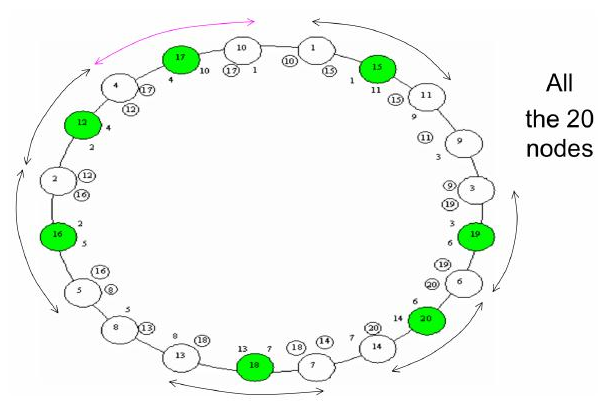
\includegraphics[width=0.95\textwidth]{figs/hs_ex0.png}
    \caption{HS Phase 0. \cite{pedersenLeaderElectionDistributed2022}}
  \end{figure}
  \note{Since everything is happening asynchronously it is quite difficult to describe since their are many different sequences it may follow. Here we assume that every phase occurs simultaneously.
  
  Description of figures. The text on right describes nodes that were alive at the start of the phase. Green nodes survive for the next phase. White ones are dead after the phase.
  
  In the first phase, every node starts its own election.
  }

\end{frame}

\begin{frame}
  \frametitle{HS algorithm: Phase 1}
  \begin{figure}
    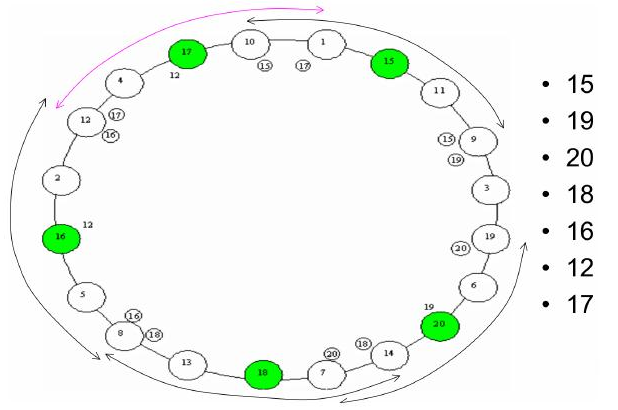
\includegraphics[width=0.95\textwidth]{figs/hs_ex1.png}
    \caption{HS Phase 1. \cite{pedersenLeaderElectionDistributed2022}}
  \end{figure}
\end{frame}

\begin{frame}
  \frametitle{HS algorithm: Phase 2}
  \begin{figure}
    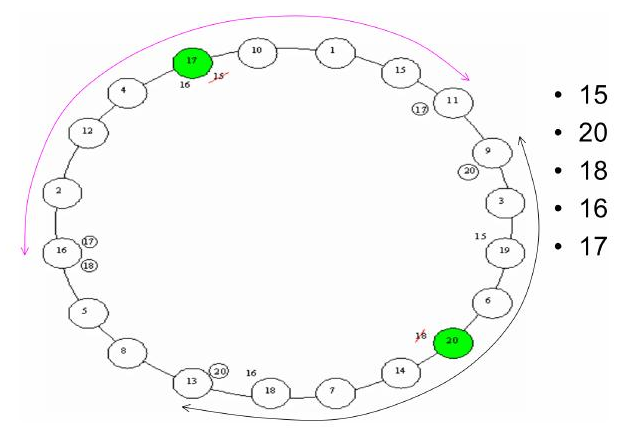
\includegraphics[width=0.95\textwidth]{figs/hs_ex2.png}
    \caption{HS Phase 2. \cite{pedersenLeaderElectionDistributed2022}}
  \end{figure}
\end{frame}

\begin{frame}
  \frametitle{HS algorithm: Phase 3}
  \begin{figure}
    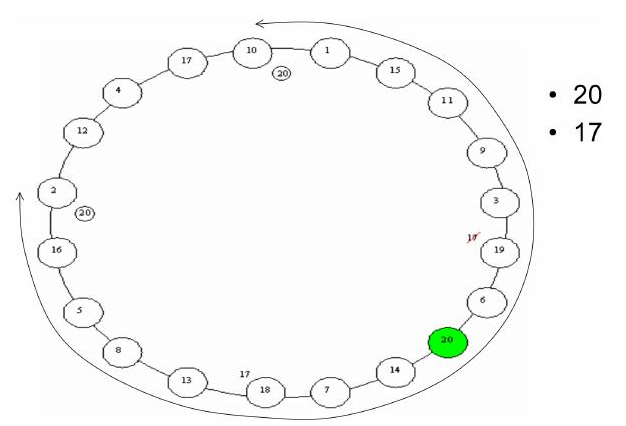
\includegraphics[width=0.95\textwidth]{figs/hs_ex3.png}
    \caption{HS Phase 3. \cite{pedersenLeaderElectionDistributed2022}}
  \end{figure}
\end{frame}

\begin{frame}
  \frametitle{HS algorithm: Phase 4}
  \begin{figure}
    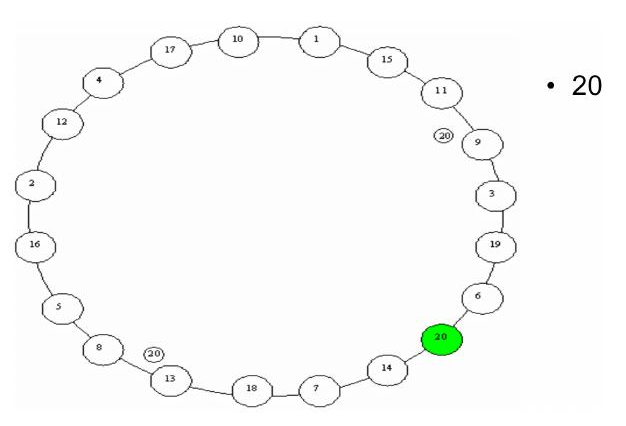
\includegraphics[width=0.95\textwidth]{figs/hs_ex4.png}
    \caption{HS Phase 4. \cite{pedersenLeaderElectionDistributed2022}}
  \end{figure}
\end{frame}

\begin{frame}
  \frametitle{HS algorithm: Phase 5}
  \begin{figure}
    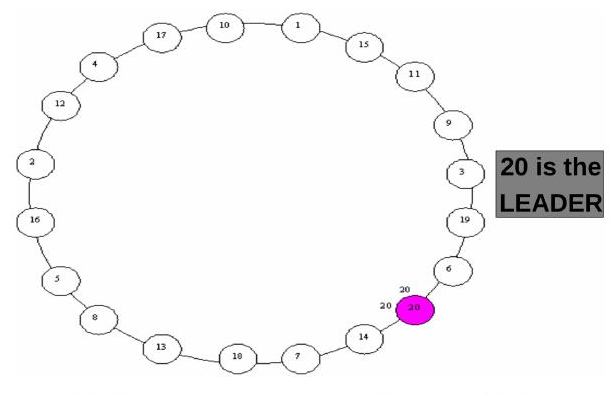
\includegraphics[width=0.95\textwidth]{figs/hs_ex5.png}
    \caption{HS Phase 5. \cite{pedersenLeaderElectionDistributed2022}}
  \end{figure}
\end{frame}

\note{
  Message complexity:

  For a single transmitter:
  \begin{itemize}
    \item Sends 1 message to one-hop neighbors and they get a response. = 4 messages.
    \item Sends to two-hop neighbors 8 messages.
    \item Sends to four-hop neighbors 16 messages.
    \item Sends to eight-hop neighbors 32 messages.
    \item Sends to sixteen-hop neighbors 64 messages.
  \end{itemize}

  This boils down to $4\cdot (1\cdot n + 2\cdot [n/2] + 4\cdot [n/3] + 8\cdot [n/5] \ldots + 2^i\cdot [n/(2^{i-1}+1)])$

  Knowing that no process will pass messages along a path greater than $2n$ the total number of messages is less than $8n + 8[n\log n)] = \mathcal{O}(n\cdot \log n)$
}

\note{
  Bemærk at ved HS algorithm er det ikke kun til node $2^k$ vi sender, det er til alle på vejen. Node 18 er et godt eksempel på dette, da den dør til node 20, selvom den ikke går op i $2^k$.
}

\section{References}
\begin{frame}[allowframebreaks]{References}
  \bibliographystyle{ieeetr}
  \bibliography{references}
\end{frame}

\end{document}
